\section{Evaluations} \label{sec:evaluation}
To evaluate the performance of the CloudCache and validate whether the cache idea is feasible in reality, we deploy the CloudCache framework to Amazon EC2 platform in a small scale (Fig.~\ref{fig:ec2}). In the deployment, there are $1$ Master Node, $4$ Slave Node/Data Node, and $1$ Sinker Node. All EC2 instances are micro which have the specifications in Table~\ref{tab:ec2}.

\begin{figure*}
\centering
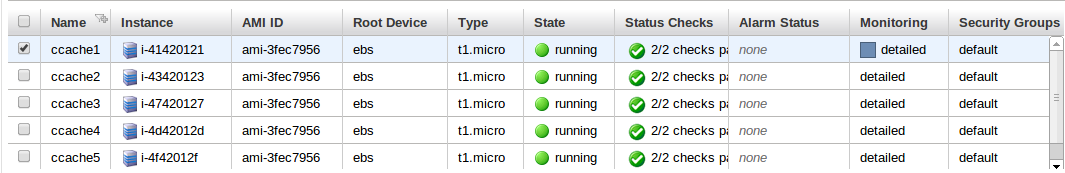
\includegraphics[width=\textwidth]{pics/deployment.png}
\caption{The EC2 instances in deployment}
\label{fig:ec2}
\end{figure*}

\begin{table}
\centering
\caption{EC2 Instance Specifications}
\begin{tabular}{ll}\toprule
Memory & $613$MB \\
Compute Units & up to $2$ \\
Operating System & Ubuntu 12.04 LTS 64-bit \\
I/O Performance & Low \\\bottomrule
\end{tabular}
\label{tab:ec2}
\end{table}

Additionally, we run a standard benchmark for Redis server on the Data Node. The results are shown in Table~\ref{tab:redis}. Two operations \emph{GET} and \emph{SET} are frequently used in CloudCache, which has the throughput of $25316.46$ and $17421.60$ requests per second respectively.

\begin{table}
\centering
\caption{Redis Server Benchmark}
\begin{tabular}{ll}\toprule
Redis Operations & Benchmark Results \\\midrule
PING & 26109.66 requests per second \\
MSET & 12406.95 requests per second \\
SET & 17421.60 requests per second \\
GET & 25316.46 requests per second \\
INCR & 24813.90 requests per second \\
LPUSH & 27700.83 requests per second \\
LPOP & 28169.02 requests per second \\
SADD & 28169.02 requests per second \\
SPOP & 27777.78 requests per second \\
LPUSH & 27855.15 requests per second \\
LRANGE & 3373.82 requests per second \\\bottomrule
\end{tabular}
\label{tab:redis}
\end{table}

Then we randomly generate $1,000,000$ 3-SAT problem instances, then the Client node submit those problem instances as a job to the Master Node. The Slave Node starts solving the problem using kernel-solver and we collect the runtime statistics for the problem solving time and cache hit rate. Further, we use the Amazon CloudWatch as the system performance monitor tool to track the CPU usage and network consumption inside the framework.

\subsection{Problem Solving Performance}
One of the major performance metrics is the problem solving time, which shows how much time to solve a problem using CloudCache framework. In this evaluation, we generate $1,000,000$ problem instances randomly whose number of variables is between $1$ and $20$ and the number of clauses is between $1$ and $256$. We solve the $1,000,000$ twice: the first time we use brute-force approach by exhaustive search, and the second time we solve it within the CloudCache framework. During the experiments, we collect the time of each problem instance, then we draw a cumulative distribution frequency curve in Fig.~\ref{fig:time}.

\begin{figure}
\centering
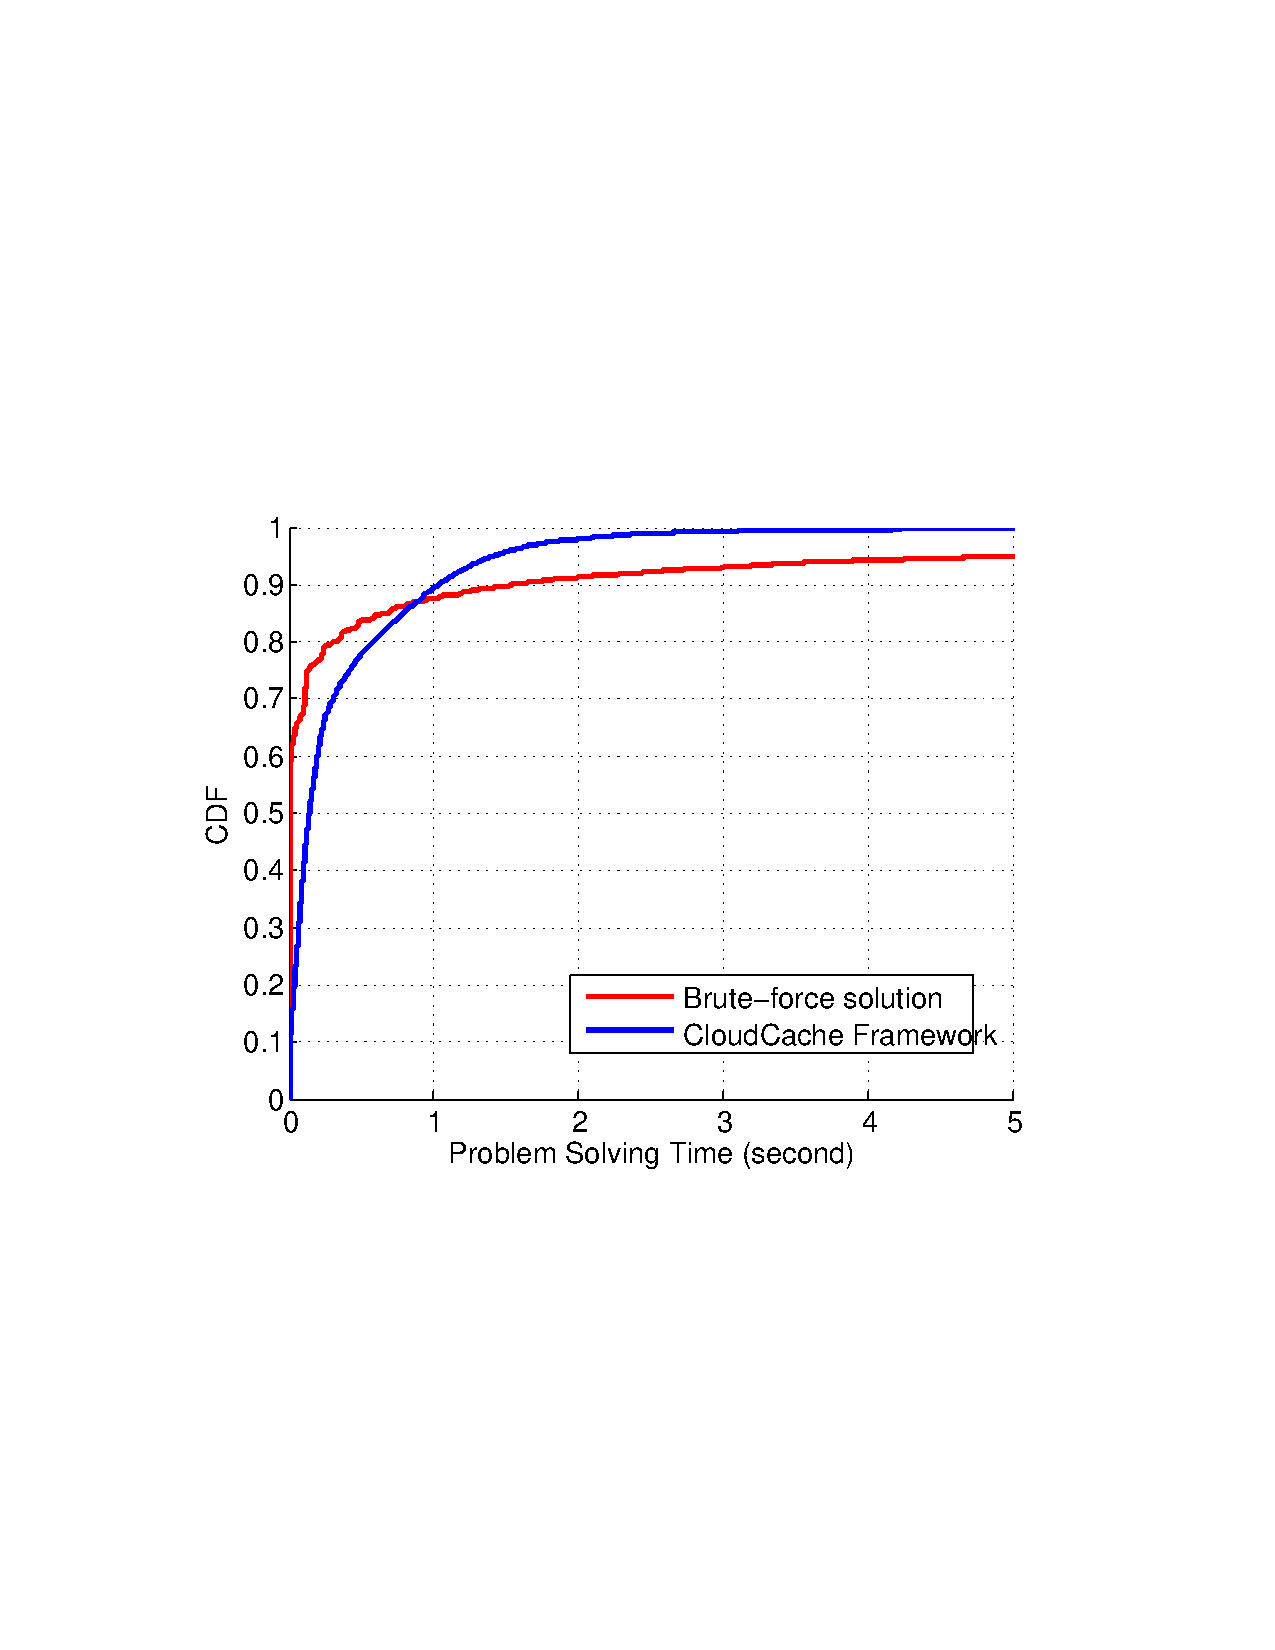
\includegraphics[width=0.45\textwidth]{pics/time.pdf}
\caption{The problem solving time CDF curve.}
\label{fig:time}
\end{figure}

As is shown in the figure, for easy problem instances, which usually can be solved within a second, brute-force approach has more advantages. However, brute-force approach cannot benefit the hard problem instances at all, while the CloudCache framework can handle it very well. We think the linear scan and cache query process cost non-trivial amount of time for easy problem instances, but this time benefits the hard problem instances by reducing the exhaustive search into a simple validation process. Finally, it is safe to say the CloudCache framework is a good fit for the hard problem instances.

\subsection{Framework Performance}
First, we look at the Master Node. Fig.~\ref{fig:master_cpu} gives the CPU performance dynamics along with the whole process. As we can see, there are only several time points that the CPU cost of the Master Node is significant which include job distribution and its TCP server. Most of the time, the CPU cost in Master Node can be ignored which gives the opportunity that the Master Node can continue accepting other job submisions. The In-network (Fig.~\ref{fig:master_in}) and out-network (Fig.~\ref{fig:master_out}) performance shows there is no long-term major network activities in the Master Node, except for the job distribution phase.

Second, we take a Slave Node's tracking results. As is shown in Fig.~\ref{fig:slave_cpu}, the Slave Node's CPU reaches to full load right after the job distribution phase of Master Node. During the next several hours, the Slave Node is busy solving problem assigned to itself. From Fig.~\ref{fig:slave_in} we can see the job receiving phase's in-network fringerprints. Once the Slave Node starts working, the out-network starts increasing because the generated solutions will be sinked to the Sinker Node. Thus, as is illustrated in Fig.~\ref{fig:slave_out}, the out-network starts busy right after the Slave Node starts working. Besides, the trends to grow in out-network indicates the problem solving throughput increases and it takes less and less time to solve a problem when we cache more and more solutions. However, the grows are sub-linear as $O(log^n)$ where $n$ is the number solutions cached. A possible reason is the EC2 instance type become a bottleneck for this framework.

Finally, the Sinker Node's CPU (Fig.~\ref{fig:sinker_cpu}) is in mild load because we adopt the solution report buffer in the Slave Node. The in-network (Fig.~\ref{fig:sinker_in}) confirms the conclusions that the framework is speeding up the problem solution as a whole, because the increase in the in-network has the same growing style with Slave Node's out-network. The Sinker Node's out-network (Fig.~\ref{fig:sinker_out}) also shows the ACKs for receiving data from TCP which has the similar shape to the in-network.

\begin{figure*}
\minipage{0.33\textwidth}
  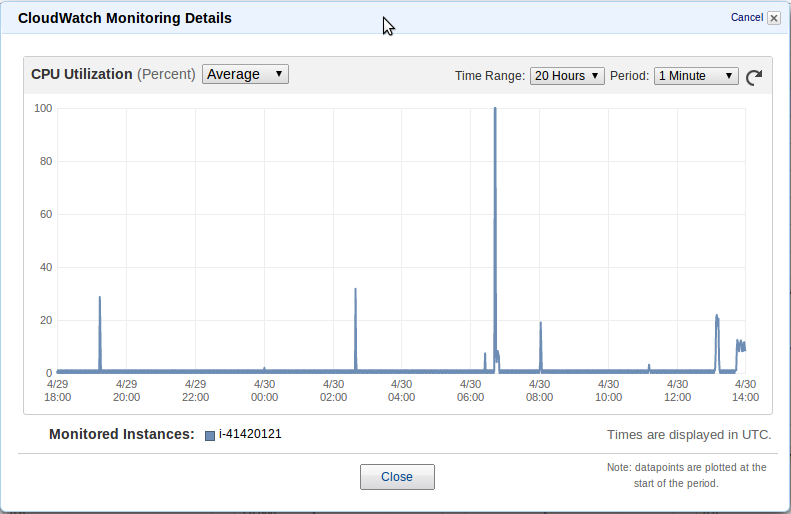
\includegraphics[width=\linewidth]{pics/master_cpu.png}
  \caption{Master Node CPU}\label{fig:master_cpu}
\endminipage\hfill
\minipage{0.33\textwidth}
  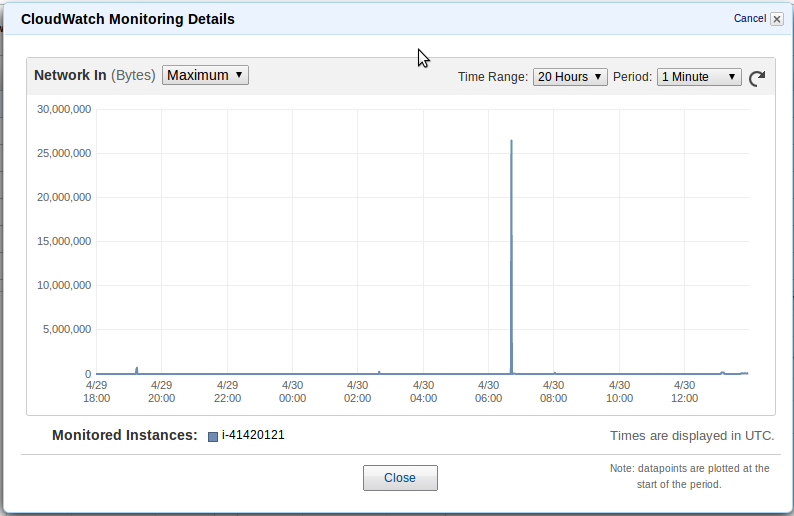
\includegraphics[width=\linewidth]{pics/master_network_in.png}
  \caption{Master Node Network In}\label{fig:master_in}
\endminipage\hfill
\minipage{0.33\textwidth}
  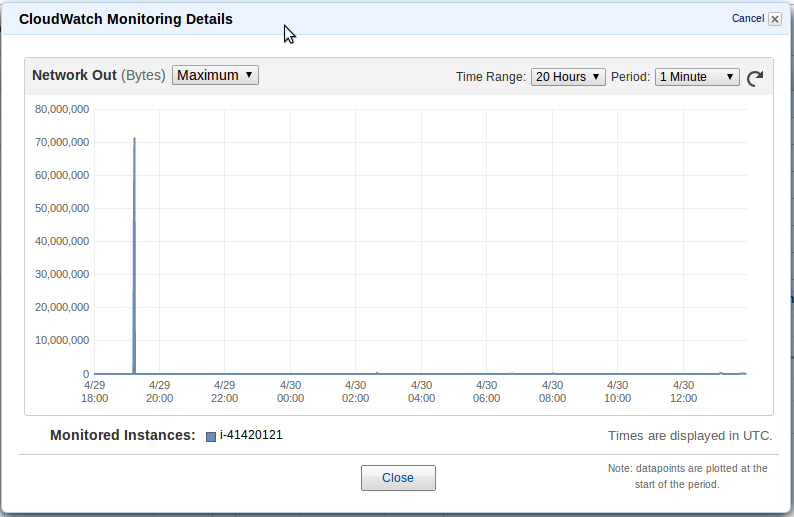
\includegraphics[width=\linewidth]{pics/master_network_out.png}
  \caption{Master Node Network Out}\label{fig:master_out}
\endminipage\hfill
\end{figure*}

\begin{figure*}
\minipage{0.33\textwidth}
  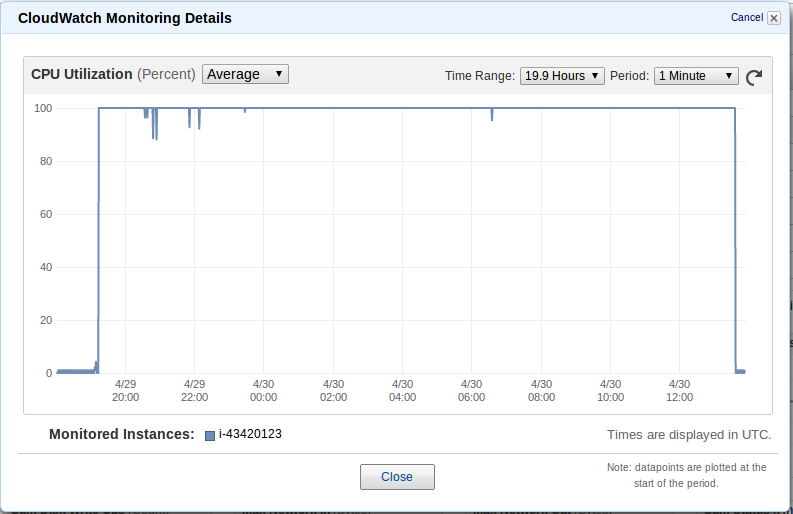
\includegraphics[width=\linewidth]{pics/slave_cpu.png}
  \caption{Slave Node CPU}\label{fig:slave_cpu}
\endminipage\hfill
\minipage{0.33\textwidth}
  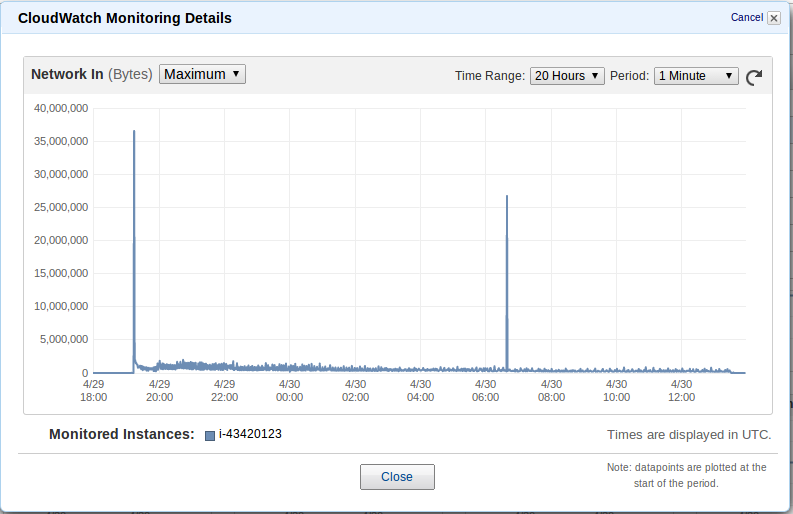
\includegraphics[width=\linewidth]{pics/slave_network_in.png}
  \caption{Slave Node Network In}\label{fig:slave_in}
\endminipage\hfill
\minipage{0.33\textwidth}
  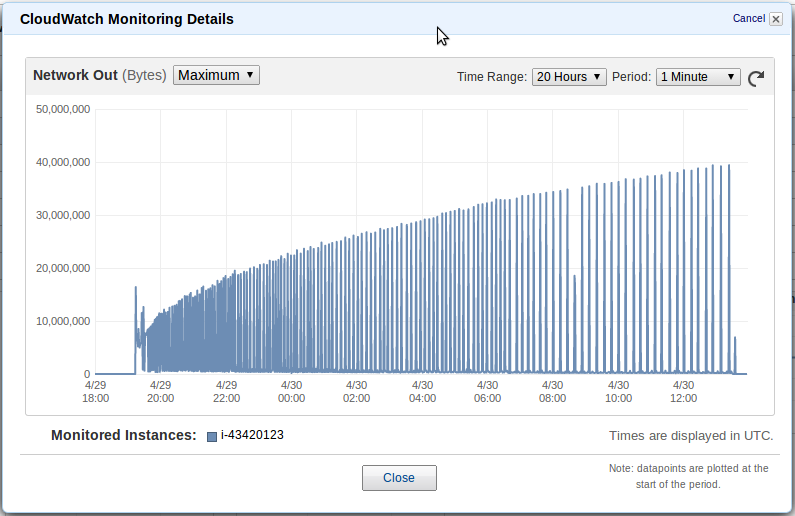
\includegraphics[width=\linewidth]{pics/slave_network_out.png}
  \caption{Slave Node Network Out}\label{fig:slave_out}
\endminipage\hfill
\end{figure*}

\begin{figure*}
\minipage{0.33\textwidth}
  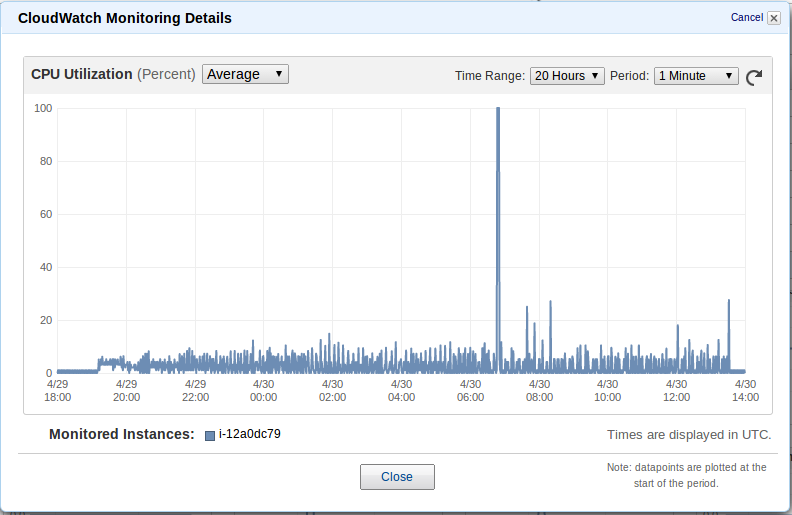
\includegraphics[width=\linewidth]{pics/sinker_cpu.png}
  \caption{Sinker Node CPU}\label{fig:sinker_cpu}
\endminipage\hfill
\minipage{0.33\textwidth}
  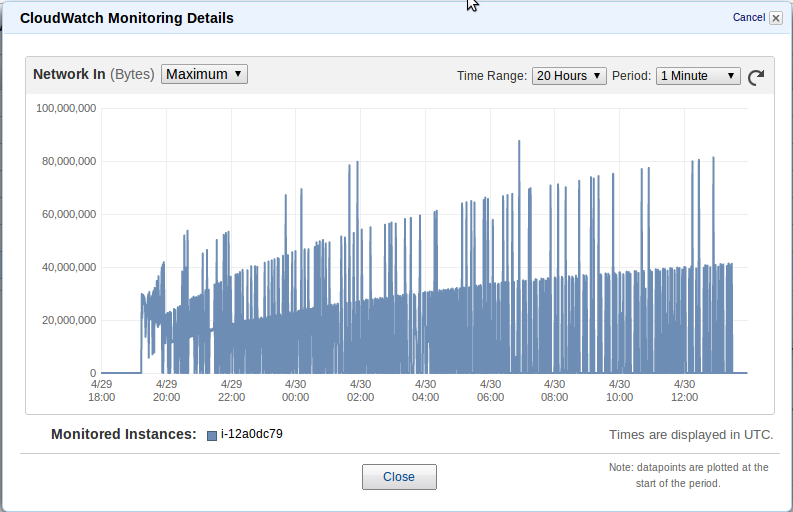
\includegraphics[width=\linewidth]{pics/sinker_network_in.png}
  \caption{Sinker Node Network In}\label{fig:sinker_in}
\endminipage\hfill
\minipage{0.33\textwidth}
  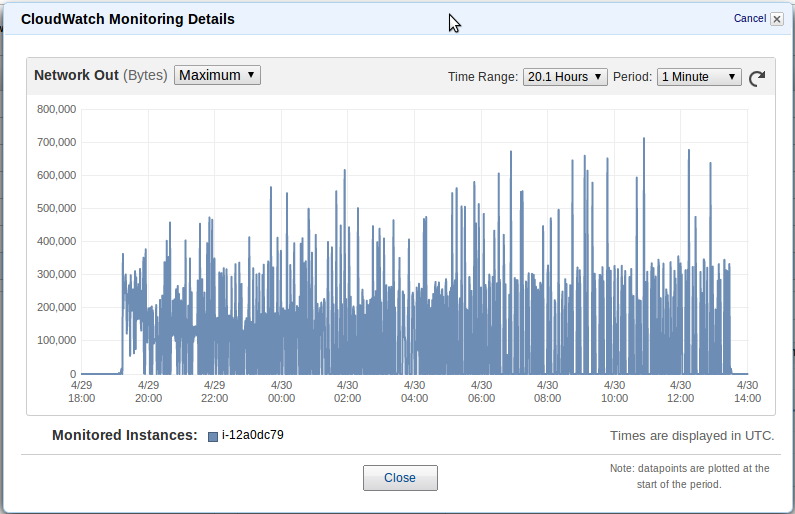
\includegraphics[width=\linewidth]{pics/sinker_network_out.png}
  \caption{Sinker Node Network Out}\label{fig:sinker_out}
\endminipage\hfill
\end{figure*}
